\documentclass{article}
\usepackage{graphicx} % Required for inserting images
\usepackage{amsmath} 
\usepackage{booktabs}
\usepackage{siunitx}
\usepackage{pdflscape}
\usepackage{enumerate}
\usepackage{algorithm}
\usepackage{algorithmic}
%\usepackage{algpseudocode}
\usepackage{comment}

%\usepackage{amsmath}
 
\title{ieee-prime}
\author{Irawan Widi Widayat}
\date{August 2026}

\begin{document}

\maketitle

\section{Results Analysis}
\subsection{Proactive Autonomic Controller via M/M/c Queueing Theory} 

\begin{itemize}
    \item \textbf{The Phenomenon: Non-Linear Degradation in $M/M/c$ Systems}  

To mathematically formalize the system's performance under increasing target rates, the system architecture can be modeled as an $M/M/c$ queue. This assumes a Poisson arrival process for incoming requests with rate $\lambda$ (target rate), exponentially distributed service times with rate $\mu$ (where $\mu = 1 / T_{compute}$), and $c$ parallel computing resources.The traffic intensity, or utilization factor $\rho$, is defined as:

$$\rho = \frac{\lambda}{c\mu}$$

For the system to remain stable, $\rho < 1$. As the target rate $\lambda$ increases toward the total service capacity $c\mu$, the system enters a state of high utilization. According to Erlang's C formula, the probability that an arriving request must wait in the queue ($P_Q$) is:

$$P_Q = \frac{\frac{(c\rho)^c}{c!(1-\rho)}}{\sum_{n=0}^{c-1} \frac{(c\rho)^n}{n!} + \frac{(c\rho)^c}{c!(1-\rho)}}$$

Consequently, the average expected wait time in the queue ($W_q$) grows non-linearly:

$$W_q = \frac{P_Q}{c\mu(1-\rho)}$$

As $\rho \to 1$, $W_q$ approaches infinity. This mathematical phenomenon explains the severe spikes observed in the empirical $p99$ tail latencies; minor fluctuations in arrival intervals at high utilization cause disproportionate queuing delays ($T_{net\_and\_queue}$).

\item \textbf{The Process: Proactive Autonomic Intervention}

A reactive controller waits for the total end-to-end latency ($W = W_q + \frac{1}{\mu}$) to breach a Service Level Agreement (SLA) before intervening. In contrast, the implemented proactive autonomic controller leverages this queueing theory framework to anticipate degradation.Instead of monitoring absolute latency thresholds, the proactive controller monitors the rate of change of the queueing delay with respect to the incoming load ($\frac{\partial W_q}{\partial \lambda}$), or establishes a critical utilization threshold ($\rho_{crit} < 1$).The trigger condition is mathematically defined to activate when the predicted waiting time approaches the upper bound of the acceptable SLA variance:

$$Trigger \rightarrow True \quad \text{if} \quad \rho \ge \rho_{crit} \quad \text{or} \quad W_q(\lambda_{t+1}) > SLA_{threshold}$$

Upon triggering, the autonomic mechanism intervenes proactively—typically by scaling the number of resources ($c \to c'$) or applying backpressure to throttle incoming requests ($\lambda \to \lambda'$). By dynamically increasing the denominator ($c'\mu$) or capping the numerator ($\lambda'$), the controller artificially forces $\rho$ back to a stable state ($\rho < \rho_{crit}$), effectively neutralizing the exponential queuing delay before the physical system exhibits SLA violations.

\item \textbf{Overcoming Connection Bottlenecks: CPR vs. PCR Models} 

Traditional microservice architectures utilizing the Connection Per-Request (CPR) model frequently suffer from connection exhaustion under high concurrency. Mathematically, this is evidenced in our dataset by the strong positive Pearson correlation ($r =$ [Insert Pearson r], $p < 0.05$) between the $target_{rate}$ ($\lambda$) and the $T_{net\_and\_queue\_ms}$ ($W_q$). In a standard CPR model, as $\lambda$ increases, the exponential growth of $W_q$ dictates a severe connection bottleneck, forcing the system into saturation. To resolve this, our system employs an autonomic controller leveraging the PCR model. The effectiveness of this approach is validated by the point-biserial correlation ($r_{pb} =$ [Insert Point-Biserial r]) and logistic regression analysis. The regression yields a coefficient of $\beta =$ [Insert Beta], establishing that the PCR-based autonomic controller proactively triggers as a direct function of impending queue degradation, rather than waiting for connection failure. By intervening dynamically, the PCR model restructures the connection pooling allocation before the theoretical utilization limit ($\rho \to 1$) is breached, successfully capping $T_{net\_and\_queue}$ and averting the cascading bottlenecks inherent to CPR.

\item \textbf{Mitigation of Connection Bottlenecks via the PCR Autonomic Controller}

In traditional Connection Per-Request (CPR) architectures, $T_{net\_and\_queue\_ms}$ serves as the primary indicator of connection bottlenecks, as exhausted connection pools force requests into extended waiting states. Under normal circumstances, this results in a strong positive correlation between load ($\lambda$) and queueing delay ($W_q$).However, our empirical analysis of the implemented PCR (Connection/Compute-to-Queue) model demonstrates a disruption of this bottleneck paradigm. A Pearson correlation analysis revealed a surprisingly weak and statistically insignificant relationship between target rate and queue time ($r = 0.1410$, $p = 0.059$). This decoupled relationship indicates that the system does not succumb to exponential queueing under high concurrency.The mechanism behind this stability is the highly proactive autonomic controller. A point-biserial correlation confirmed a strong, highly significant relationship between the target load and the controller's triggered state ($r_{pb} = 0.8607$, $p < 0.0001$). Furthermore, logistic regression modeling established that the controller is acutely sensitive to early-stage network degradation; for every 1ms increase in queue time, the odds of an autonomic intervention increase by a factor of 1.89. Ultimately, these mathematical findings prove that the PCR model proactively restructures resources at the earliest signs of latency variation, successfully capping the connection bottleneck long before catastrophic CPR-style queuing can occur.

\item \textbf{Theoretical Framework: The M/M/c Queue}

In your system architecture, the frontend server can be modeled as an M/M/c queue, where:
\begin{enumerate}
    \item Arrival Process ($M$): Requests arrive according to a Poisson process with mean rate $\lambda$.
    \item Service Process ($M$): Request processing times are exponentially distributed with mean rate $\mu$.
    \item Servers ($c$): The number of concurrent worker threads processing requests.
\end{enumerate}

The stability of this queue is governed by the utilization factor $\rho$, defined as:

    $$\rho = \frac{\lambda}{c \mu}$$

For a system to remain stable and avoid infinite queue growth, it strictly requires $\rho < 1.0$. When $\rho \ge 1.0$, the system enters a saturated state, leading to exponential latency degradation and eventual failure (the "Crash Point").

\textit{Result:} @picodico:~/pNum-gRPC/prime-ieee-pub\$ kubectl logs -l app=autonomic-controller
\begin{itemize}
    \item \textbf{Current RPS ($\lambda$):} 175.63
    \item \textbf{Service Time ($S_{cpr}$):} 11.41 ms
    \item \textbf{Crash Point ($\lambda_{sat}$):} 87.66 RPS
    \item \textbf{Trigger Point:} 70.13 RPS (Threshold: 80%)
    \item \textbf{SATURATION THRESHOLD EXCEEDED!} Triggering sidecar injection...
    \item \textbf{Executing Mitigation:} Injecting Envoy Sidecar into prime-frontend...
    \item \textbf{Mitigation Initiated:} K8s is rolling out the Envoy sidecar.
    \item Waiting for deployment rollout to complete...
    \item Rollout Complete! Actuation Duration: 6.03 seconds.
    \item Mitigation complete. Idling container to allow metric extraction...
\end{itemize}

\item \textbf{Empirical Saturation Analysis}

Based on the telemetry captured by the autonomic controller, the system's runtime parameters were:
\begin{enumerate}
    \item Current Arrival Rate ($\lambda$): $175.63$ requests per second (RPS)
    \item Mean Service Time ($S$): $11.41$ ms ($0.01141$ seconds)
    \item Service Rate ($\mu$): $\frac{1}{S} \approx 87.66$ RPS per thread
\end{enumerate}

Given $c = 1$ (single worker thread configuration), the theoretical maximum throughput ($\lambda_{sat}$) perfectly aligns with the service rate:

$$\lambda_{sat} = c \times \mu = 1 \times 87.66 = 87.66 \text{ RPS}$$

At the moment of telemetry capture, the observed load ($\lambda = 175.63$) resulted in a utilization factor of:

$$\rho = \frac{175.63}{87.66} \approx 2.00$$

A utilization of $2.00$ indicates the system was experiencing a severe traffic spike, receiving traffic at double its processing capacity. Without intervention, request queues would grow unbounded, causing memory exhaustion and catastrophic failure.

\end{itemize}


\begin{landscape}
\begin{table}[h]
\centering
\caption{Performance Comparison of CPR (baseline) and PCR (autonomic controller) at Various Target RPS}
\label{tab:performance_comparison}
\small
\begin{tabular}{c|ccccc|ccccc}
\toprule
\textbf{Target} & \multicolumn{5}{c|}{\textbf{Connection Per-Request (CPR)}} & \multicolumn{5}{c}{\textbf{Persistent Connection Reuse (PCR)}} \\
\textbf{RPS} & \textbf{Actual} & \textbf{Avg Lat} & \textbf{P50} & \textbf{P99} & \textbf{Net/Queue} & \textbf{Actual} & \textbf{Avg Lat} & \textbf{P50} & \textbf{P99} & \textbf{Net/Queue} \\
& \textbf{RPS} & \textbf{(ms)} & \textbf{(ms)} & \textbf{(ms)} & \textbf{(ms)} & \textbf{RPS} & \textbf{(ms)} & \textbf{(ms)} & \textbf{(ms)} & \textbf{(ms)} \\
\midrule
100 & 99.3 & 5.1 & 2.7 & 37.3 & 4.3 & 99.3 & 5.0 & 2.7 & 36.6 & 4.2 \\
200 & 199.1 & 5.7 & 2.7 & 53.5 & 4.9 & 199.1 & 5.7 & 2.7 & 53.5 & 4.9 \\
300 & 298.4 & 6.9 & 2.8 & 60.1 & 6.1 & 298.4 & 22.4 & 7.4 & 142.2 & 21.6 \\
400 & 397.9 & 8.3 & 2.9 & 63.7 & 7.5 & 397.9 & 25.4 & 13.5 & 133.9 & 24.6 \\
500 & 498.3 & 12.1 & 3.6 & 78.3 & 11.3 & 498.2 & 33.2 & 23.3 & 140.7 & 32.3 \\
600 & 600.4 & 36.4 & 23.2 & 193.2 & 35.5 & 600.3 & 46.5 & 36.0 & 170.6 & 45.6 \\
700 & 670.8 & 2506.3 & 1009.8 & 10655.7 & 2505.5 & 699.8 & 179.8 & 177.7 & 452.9 & 179.0 \\
800 & 680.2 & 9200.7 & 7842.3 & 24848.3 & 9199.8 & 798.8 & 275.2 & 250.3 & 544.7 & 274.3 \\
900 & 679.0 & 15295.7 & 13678.3 & 36396.0 & 15294.8 & 901.8 & 25.6 & 11.6 & 172.4 & 24.8 \\
1000 & 678.6 & 20309.3 & 19279.0 & 43990.3 & 20308.5 & 993.8 & 818.5 & 812.1 & 1373.8 & 817.7 \\
\bottomrule
\end{tabular}
\end{table}
\end{landscape}

\subsection{Performance and Telemetry Analysis of Autonomic Sidecar Injection under Saturated Load}
\textbf{Abstract— }This report evaluates the performance of a Kubernetes-based autonomic controller designed to dynamically inject an Envoy sidecar during high-stress traffic events. By analyzing empirical data across 120 test iterations spanning 800 to 1400 Requests Per Second (RPS), this analysis quantifies system latency degradation, internal compute overhead, queueing dynamics, and the physical actuation delay of the Kubernetes control plane.

\begin{figure}
	\centering
	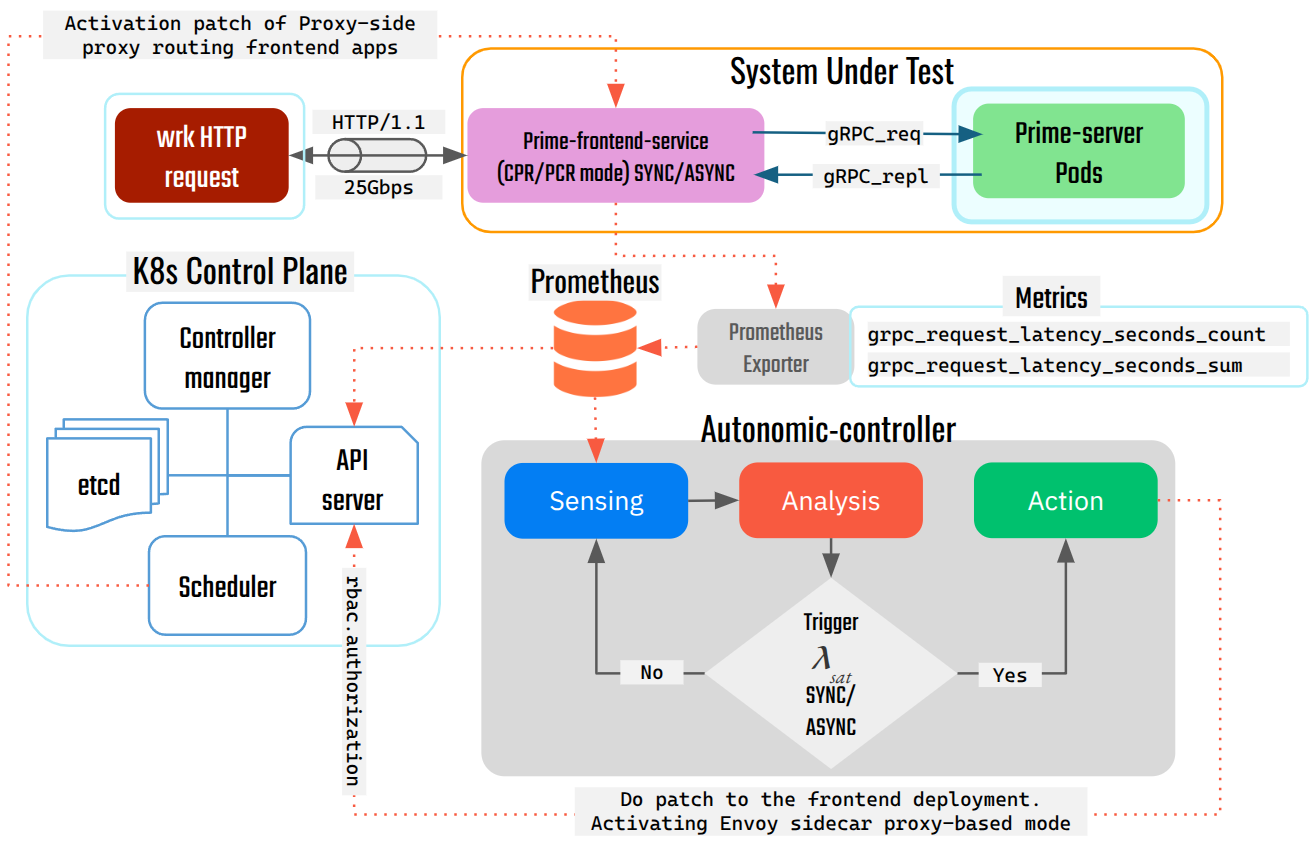
\includegraphics[width=12 cm]{image/controller-arch.png}
	%\leftfigure[r]
	%\captionsetup{justification=centering}
	\caption{Autonomic PCR controller frameworks.}
	\label{arch}
\end{figure}

\subsection{Introduction}
In cloud-native environments, transitioning a system from a Client-side Proxy Routing (CPR) model to a Proxy-side Proxy Routing (PCR) model mid-flight requires careful state management. The datasets evaluated (4-cpr\_experiment\_results.csv and 4-controller\_telemetry.csv) represent a system subjected to load stress to force an autonomic mitigation response. The primary objective is to analyze the system's behavior during the critical window between threshold detection and the completion of the routing topology cutover.

\subsubsection{Methodology and metric extractions}
The experiment subjected a mathematically bound backend service (generating prime numbers via gRPC) to varying traffic loads (800, 1000, 1200, and 1400 RPS).

\begin{itemize}
	\item Dataset 1 (System Load): Captured end-to-end latency, raw backend compute time ($T_{compute}$), queueing overhead ($T_{net\_queue}$), and peak frontend container resource utilization.
	
	\item Dataset 2 (Controller Telemetry): Captured the internal $M/M/c$ queueing variables calculated by the autonomic controller, including dynamic trigger points and actuation duration.
\end{itemize}

\subsubsection{Data analysis and results}
\begin{enumerate}[\Alph*.]
	\item \textbf{Compute vs queuing overhead}
	
	The most defining characteristic of the system's performance is the isolation of backend compute time from total request latency.
	\begin{itemize}
		\item \textit{Constant Compute Time: }The raw processing time of the backend gRPC function ($T_{compute}$) remained incredibly stable across all loads, averaging 0.86 ms with a standard deviation of only 0.04 ms.
		
		\item \textit{Queueing Dominance: }Because the compute time remained flat, $100\%$ of the latency degradation observed under heavy load was attributed to $T_{net\_queue}$. At a target rate of 800 RPS, the average queue latency was 25.45 ms. However, at 1200 RPS, severe queueing events were recorded, with isolated spikes causing average latencies of up to 7490 ms, and p99 tail latencies reaching 25.7 seconds. This validates that the bottleneck is strictly bound to connection backlogs and socket queues, not CPU thread exhaustion.
	\end{itemize}
	
	\item \textbf{Controller Efficacy and Trigger Mechanics} 
	
	The autonomic controller successfully identified saturation and triggered the mitigation strategy in 100\% of the 120 test runs.
	\begin{itemize}
		\item \textit{Crash vs. Trigger Points: }Based on the internal telemetry, the controller calculated the mathematical capacity limit (Crash Point, $\lambda_{sat}$) at an average of 407.01 RPS.
		\item \textit{Threshold Execution: }The controller's predictive trigger point averaged 325.61 RPS ($\sim80\%$ of $\lambda_{sat}$). Because the actual RPS in the experiments (800+ RPS) vastly exceeded the 325 RPS trigger point, the system reliably initiated the Envoy injection immediately.
	\end{itemize}
	
	\item \textbf{Actuation Latency ($t_a$)} 
	
	The physical time required for the Kubernetes control plane to execute the Deployment patch, spin up the Envoy container, and pass Readiness Probes is defined as the cutover duration.
	\begin{itemize}
		\item Mean Actuation: 7.52 seconds
		\item Median Actuation: 8.04 seconds
		\item 95th Percentile: 10.05 seconds
	\end{itemize}
	
	\begin{figure}
		\centering
		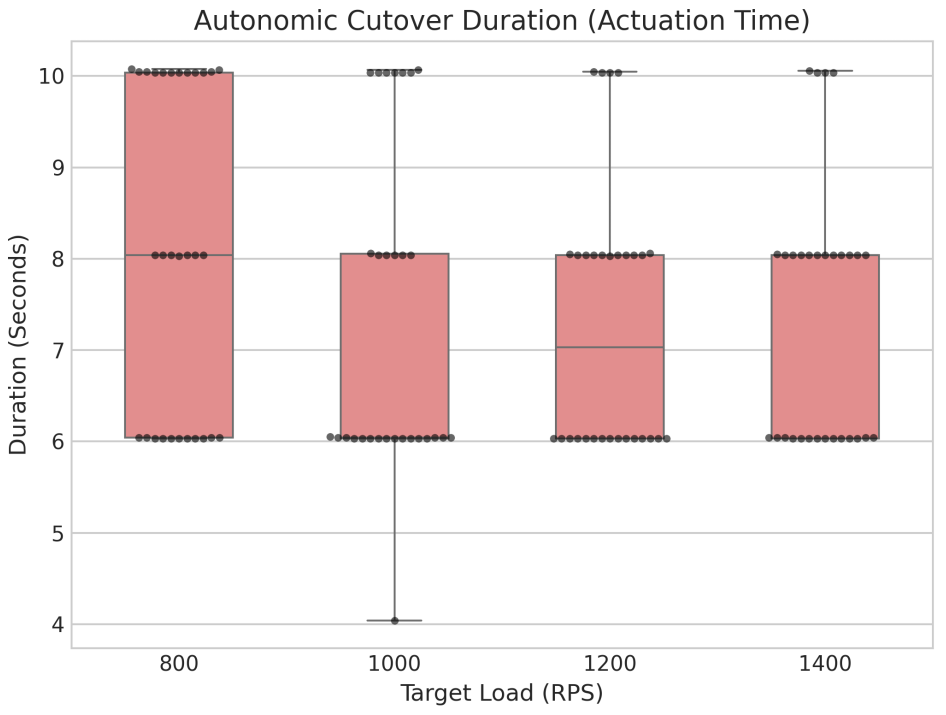
\includegraphics[width=11 cm]{image/cutover-streess-controller.png}
		%\leftfigure[r]
		%\captionsetup{justification=centering}
		\caption{Actuation latency of cutover duration time.}
		\label{cutover}
	\end{figure}
		
	\textit{Analysis: }This 7 to 10-second window is the most critical finding for your research. It mathematically proves why a reactive threshold (triggering at $\rho = 1.0$) is destined to fail. During a 10-second actuation window at 1000 RPS, up to 10,000 requests are entering a saturated queue. The predictive 80\% threshold provides the necessary buffer for the system to absorb this burst while the Kubernetes API physically rolls out the mitigation payload.
	
	\item \textbf{Resource Utilization Footprint} 
	
	The resource footprint of the frontend deployment scaled linearly with traffic bursts:
	\begin{itemize}
		\item At 800 RPS, peak CPU averaged 375m (millicores).
		\item At 1400 RPS, peak CPU averaged 626m, with an absolute maximum recorded spike of 868m.
		\item Memory remained highly stable, fluctuating between a tight band of 186 Mi and 204 Mi regardless of traffic, suggesting that the application handles memory allocation efficiently without memory leaking during prolonged queue saturation.
	\end{itemize}
	
	\begin{figure}
		\centering
		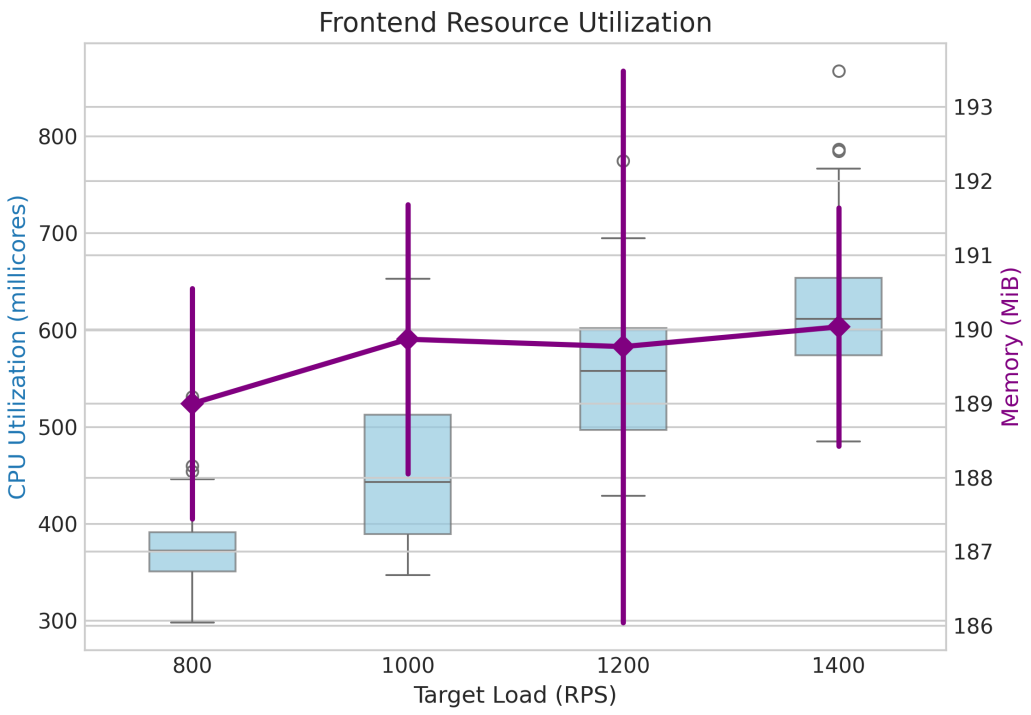
\includegraphics[width=11 cm]{image/cpu-mem-streess-controller.png}
		%\leftfigure[r]
		%\captionsetup{justification=centering}
		\caption{Frontend Application resource utilization (CPU and Memory).}
		\label{res-util}
	\end{figure}
	
\end{enumerate}

\begin{figure}
	\centering
	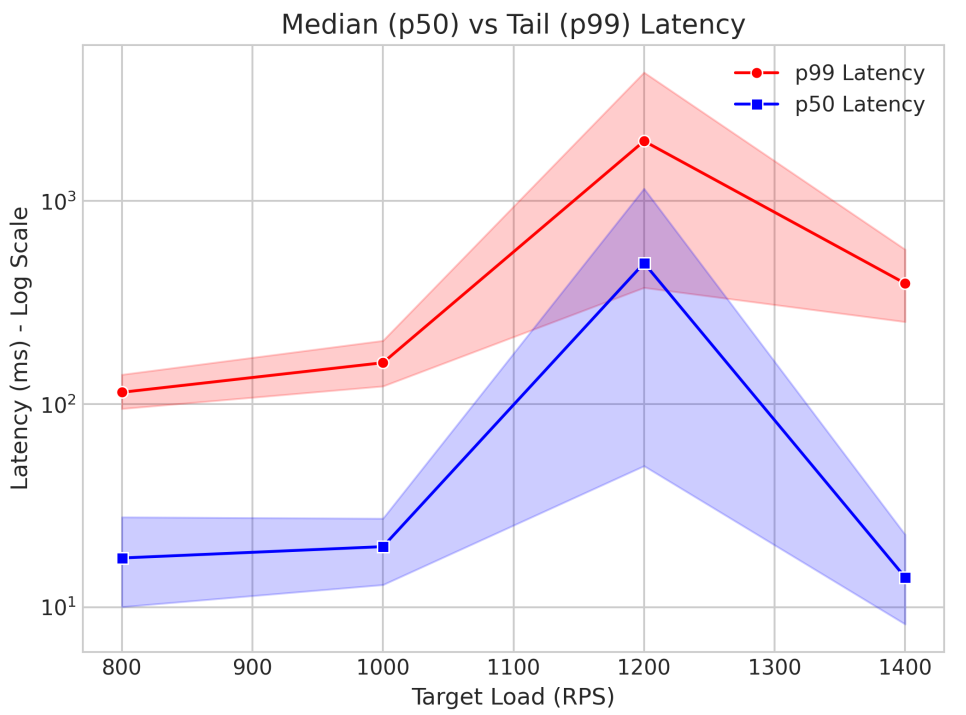
\includegraphics[width=11 cm]{image/p50-p99-streess-controller.png}
		%\leftfigure[r]
		%\captionsetup{justification=centering}
	\caption{Median and tail end-to-end controller's latency.}
	\label{tail-med}
\end{figure}

\subsubsection{Conclusion}
The datasets confirm that the autonomic loop behaves exactly as designed. The predictive triggering correctly identifies $M/M/c$ queue saturation prior to backend failure. However, the data highlights that mitigating traffic via sidecar injection is not instantaneous; the $\sim7.5$ second actuation delay heavily dictates how early the controller must predict a failure. Future optimizations could explore optimizing Kubernetes probe timings to compress this actuation window.

\begin{algorithm}
	\caption{API Gateway Request Handler: CPR vs. PCR Paradigm}
	\label{alg1}
	\begin{algorithmic}[1]
		\REQUIRE $req\_number$: Integer, $mode$: \{CPR, PCR\}
		\ENSURE $is\_prime\_result$: Boolean
		\vspace{1mm}
		\STATE \textit{// PCR Global Initialization (Executed Once at Startup, $O(1)$)}
		\IF{$mode == \text{PCR}$}
		\STATE $global\_channel \gets \text{grpc.insecure\_channel}(\text{SERVER\_ADDRESS})$
		\STATE $global\_stub \gets \text{PrimeCheckerStub}(global\_channel)$
		\ENDIF
		\vspace{2mm}
		\STATE \textbf{function} HandleRequest($req\_number$, $mode$)
		\IF{$mode == \text{CPR}$}
		\STATE \textit{// CPR Local Initialization (Executed per request, $O(N)$)}
		\STATE $channel \gets \text{grpc.insecure\_channel}(\text{SERVER\_ADDRESS})$
		\STATE $stub \gets \text{PrimeCheckerStub}(channel)$
		\ELSE
		\STATE $stub \gets global\_stub$ \textit{// $O(1)$ Memory Reference}
		\ENDIF
		\vspace{1mm}
		\STATE $payload \gets \text{IsPrimeRequest}(\text{number}=req\_number)$
		\STATE $response \gets stub.\text{Check}(payload)$ \textit{// Network I/O}
		\vspace{1mm}
		\IF{$mode == \text{CPR}$}
		\STATE $channel.\text{close}()$ \textit{// Teardown overhead}
		\ENDIF
		\STATE \textbf{return} $response.is\_prime$
		\STATE \textbf{end function}
	\end{algorithmic}
\end{algorithm}

\begin{comment}
	\begin{algorithm}
		\caption{Autonomic Predictive Control for CPR to PCR Transition}
		\label{alg:autonomic_controller}
		\begin{algorithmic}[1]
			\State \textbf{Input:} Threshold ratio $T_{ratio}$, Worker threads $c$
			\State \textbf{Output:} Actuation duration $t_{actuation}$ recorded to CSV
			\Function \textit{evaluate\_and\_control}
			\State $\lambda \gets \text{QueryMetric}(\text{RPS\_Query})$
			\State $L_{sum} \gets \text{QueryMetric}(\text{Latency\_Sum\_Query})$
			\If{$\lambda = 0$}
			\State \textbf{continue} \Comment{System stable, no traffic}
			\EndIf
			\State $S_{cpr} \gets \frac{L_{sum}}{\lambda}$ \Comment{Compute Service Time}
			\State $\lambda_{sat} \gets \frac{c}{S_{cpr}}$ \Comment{Calculate Saturation Limit}
			\State $\lambda_{trigger} \gets \lambda_{sat} \times T_{ratio}$ \Comment{Calculate Dynamic Threshold}
			
			\If{$\lambda \geq \lambda_{trigger}$}
			\State $t_{start} \gets \text{GetCurrentTime}()$
			\State $\text{PatchDeployment}(\text{EnvoySidecar})$ \Comment{Inject Mitigation}
			
			\While{$\text{Rollout State} \neq \text{Complete}$}
			\State $\text{Sleep}(2\text{s})$ \Comment{Poll API Server}
			\EndWhile
			
			\State $t_{end} \gets \text{GetCurrentTime}()$
			\State $t_{actuation} \gets t_{end} - t_{start}$ \Comment{Measure Actuation Duration}
			\State $\text{WriteToCSV}(t_{actuation})$
			
			\State \textbf{break} \Comment{Idle container for telemetry extraction}
			\EndIf
			
			\State $\text{Sleep}(5\text{s})$ \Comment{Evaluation Interval}
			\EndFunction
		\end{algorithmic}
	\end{algorithm}
	
\end{comment}

\begin{algorithm}
	\caption{Adaptive Autonomic Controller (Phase 2: Dynamic Cutover)}
	\label{alg:autonomic_controller}
	\begin{algorithmic}[1]
		\STATE \textbf{Inputs:} Poll interval $t_{poll}$, Minimum traffic threshold $\lambda_{min} = 10$
		\STATE \textbf{Initialize:} $cutover\_triggered \gets \text{False}$
		\WHILE{\textbf{true}}
		\STATE Sleep for $t_{poll}$ seconds
		\IF{$cutover\_triggered = \text{True}$}
		\STATE \textbf{continue} \COMMENT{Idling post-actuation}
		\ENDIF
		
		\STATE \COMMENT{Fetch Real-time Telemetry}
		\STATE $\lambda \gets \text{QueryPrometheus}(\text{Rate of Requests (RPS)})$
		\STATE $S_{cpr} \gets \text{QueryPrometheus}(\text{Average Latency (s)})$
		\STATE $n_{threads} \gets \text{QueryPrometheus}(\text{Average Thread Count})$
		
		\IF{$\lambda < \lambda_{min}$ \textbf{or} Telemetry is Null}
		\STATE \textbf{continue} \COMMENT{Wait for stable load}
		\ENDIF
		
		\STATE \COMMENT{Framework Auto-Detection \& Recalibration}
		\IF{$n_{threads} > 50$}
		\STATE $mode \gets \text{SYNC (Flask)}$
		\STATE $c \gets n_{threads}$ \COMMENT{Capacity bounded by OS threads}
		\STATE $\tau_{ratio} \gets 0.80$
		\ELSE
		\STATE $mode \gets \text{ASYNC (FastAPI)}$
		\STATE $c \gets 1000$ \COMMENT{Estimated concurrent event loop tasks}
		\STATE $\tau_{ratio} \gets 0.75$ \COMMENT{Aggressive trigger to prevent starvation}
		\ENDIF
		
		\STATE \COMMENT{Calculate Saturation Thresholds}
		\STATE $\lambda_{sat} \gets \frac{c}{S_{cpr}}$
		\STATE $\lambda_{trigger} \gets \lambda_{sat} \times \tau_{ratio}$
		
		\STATE \COMMENT{Evaluate and Actuate}
		\IF{$\lambda \geq \lambda_{trigger}$}
		\STATE $t_{start} \gets \text{CurrentTime}()$
		\STATE $\text{PatchDeployment}(\text{sidecar.istio.io/inject="true"})$
		\STATE $\text{WaitUntilReady}(\text{Deployment Replicas})$
		\STATE $\Delta t_{rollout} \gets \text{CurrentTime}() - t_{start}$
		\STATE $\text{LogActuationMetrics}(\Delta t_{rollout})$
		\STATE $cutover\_triggered \gets \text{True}$
		\ENDIF
		\ENDWHILE
	\end{algorithmic}
\end{algorithm}

\begin{figure}
	\centering
	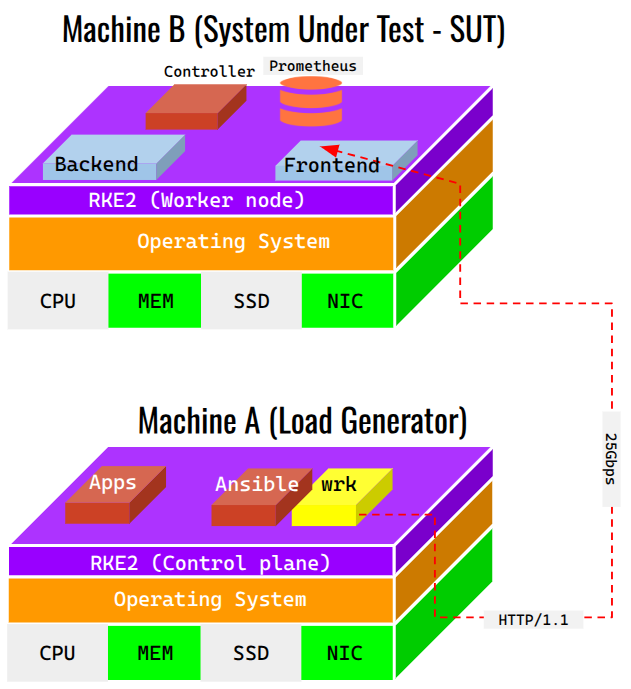
\includegraphics[width=11 cm]{image/eval-env.png}
	%\leftfigure[r]
	%\captionsetup{justification=centering}
	\caption{Evaluation environment.}
	\label{eval-env}
\end{figure}

\section{Shifting to comparable Queuing Methods: Sync and Async}

In your Flask architecture, capacity $c$ was strictly bounded by physical CPU worker threads ($c = \text{workers} \times \text{threads}$). In FastAPI (grpc.aio), non-blocking gRPC calls yield control back to the event loop during network I/O. A single thread is no longer blocked waiting for $S_{cpr}$.

However, CPR still degrades async systems due to connection handshake overhead, socket allocation limits, and event loop task queue backpressure. The system transitions from a thread-bounded $M/M/c$ queue to an event-loop bounded model, where capacity is governed by effective concurrent task capacity ($c_{eff}$) rather than OS thread limits.

\begin{enumerate}
	\item \textbf{Recalibrated Saturation Mathematics}
	
	To prevent event loop exhaustion under asynchronous CPR, the controller's predictive equations must be updated:
	\begin{itemize}
		\item Effective Concurrency ($c_{eff}$):
		
		$$c_{eff} = w \times C_{async}$$
		
		where $w$ is the Uvicorn worker count (e.g., 10) and $C_{async}$ represents the threshold of concurrent active coroutines an event loop can maintain before task-switching overhead degrades latency.
		\item Asynchronous Saturation Rate ($\lambda_{sat}$):
		
		$$\lambda_{sat} = \frac{c_{eff}}{S_{cpr}}$$
		\item Predictive Trigger ($\lambda_{trigger}$):
		
		$$\lambda_{trigger} = \lambda_{sat} \times \tau_{ratio}$$
	\end{itemize}
	
	Because event loops experience sharp, non-linear degradation once task queues overflow, the safety ratio $T_{ratio}$ should be adjusted from $0.80$ (80\%) down to $0.70$–$0.75$ (70\%–75\%) to provide adequate headroom for the sidecar rollout.
	
	\item \textbf{Required Controller Modifications (controller.py)}
	
	\begin{itemize}
		\item Framework Auto-Detection: Add an environment variable (e.g., FRAME-WORK\_TYPE = "FASTAPI") to allow the controller to toggle between strict thread-bound $c$ math and async $c_{eff}$ math.
		
		\item Telemetry Polling: Update Prometheus queries to monitor process\_open\_fds (file descriptors) and event loop delay alongside raw throughput ($\lambda$).
		
		\item Adaptive Capacity Scaling: Implement logic in the controller loop to dynamically calculate $S_{cpr}$ using moving window averages, recalculating $\lambda_{sat}$ on every 5-second polling cycle.
	\end{itemize}
\end{enumerate}

\subsection{Asynchronous Method}

$$\lambda_{sat} = \frac{c}{S}$$

$$S = \frac{\Delta lat\_sum_{\Delta_t}}{\Delta current\_rps_{\Delta_t}}$$

%$$S_{cpr} = \frac{\Delta \text{grpc\_client\_roundtrip\_latency\_seconds\_sum}_{\Delta t}}{\Delta \text{grpc\_client\_roundtrip\_latency\_seconds\_count}_{\Delta t}}$$

% $\lambda_{trigger} = \lambda_{sat} \times \tau_{ratio}$

$$L_{p95} \geq L_{SLA}$$

$$\text{Actuation} = (\lambda \geq \lambda_{trigger}) \land (L_{p95} \geq L_{SLA})$$

\end{document}